\documentclass[11pt]{article}

% --- packages ---
\usepackage[utf8]{inputenc}
\usepackage[T1]{fontenc}
\usepackage{amsmath,amssymb,amsfonts}
\usepackage{graphicx}
\usepackage{booktabs}
\usepackage{hyperref}
\usepackage{cleveref}
\usepackage[margin=1in]{geometry}
\usepackage{listings}
\usepackage{xcolor}
\usepackage{natbib}
\usepackage{tikz}
\usetikzlibrary{arrows.meta, positioning, calc}
\crefname{lstlisting}{Listing}{Listings}
\Crefname{lstlisting}{Listing}{Listings}

% --- code listing style ---
\definecolor{codebg}{RGB}{245,245,245}
\definecolor{codegreen}{RGB}{0,128,0}
\definecolor{codepurple}{RGB}{128,0,128}
\lstset{
    basicstyle=\ttfamily\small,
    backgroundcolor=\color{codebg},
    keywordstyle=\color{blue},
    stringstyle=\color{codepurple},
    commentstyle=\color{codegreen},
    numbers=left,
    numberstyle=\tiny\color{gray},
    frame=single,
    breaklines=true,
    captionpos=b
}

% --- metadata ---
\title{\texttt{BSTModelKit.jl}: A Julia Package for Constructing, Solving, and Analyzing Biochemical Systems Theory Models}
\author{
    Jeffrey D. Varner\thanks{Corresponding author: \href{mailto:jdv27@cornell.edu}{jdv27@cornell.edu}} \\
    \textit{Robert Frederick Smith School of Chemical and Biomolecular Engineering} \\
    \textit{Cornell University, Ithaca, NY 14853, USA}
}
\date{}

\begin{document}
\maketitle

% ============================================================================ %
\begin{abstract}
We present \texttt{BSTModelKit.jl}, an open-source Julia package for constructing, solving, and analyzing Biochemical Systems Theory (BST) models of biochemical networks. The package implements S-system representations, a canonical power-law formalism for modeling metabolic and regulatory networks. \texttt{BSTModelKit.jl} provides a declarative model specification format, dynamic simulation via ordinary differential equation (ODE) integration, steady-state computation, and global sensitivity analysis using the Morris and Sobol methods. The package leverages the Julia scientific computing ecosystem, in particular the SciML suite of differential equation solvers, to provide efficient and flexible model analysis tools. We describe the mathematical formulation, software design, and demonstrate the package capabilities with illustrative examples.
\end{abstract}

\noindent\textbf{Keywords:} biochemical systems theory, S-system, power-law formalism, Julia, systems biology, metabolic modeling

% ============================================================================ %
\section{Introduction}\label{sec:introduction}
Mathematical modeling of biochemical networks is essential for understanding the complex dynamics of living systems. Among the many formalisms available, Biochemical Systems Theory (BST) occupies a distinctive position: it provides a canonical mathematical structure grounded in a power-law approximation of enzyme kinetics that is both analytically tractable and broadly applicable. BST was introduced by Savageau in a series of foundational papers \citep{Savageau1969a,Savageau1969b,Savageau1970} and later elaborated in a comprehensive monograph \citep{Savageau1976}. The key insight underlying BST is that, in the vicinity of an operating point, the net rate of production or consumption of any biochemical species can be well-approximated by a product of power-law functions of the concentrations of the species in the system. This approximation is exact for mass-action kinetics and provides a remarkably good local representation of more complex rate laws, including Michaelis-Menten and Hill-type kinetics \citep{Savageau1976,Voit2000}.

The power-law formalism gives rise to two canonical representations: the Generalized Mass Action (GMA) system, which retains individual reaction terms, and the S-system, which aggregates all production and consumption terms for each species into single power-law expressions \citep{Savageau1987}. The S-system representation has particularly attractive mathematical properties---its steady-state equations can be transformed into a system of linear algebraic equations in logarithmic coordinates, enabling efficient analytical and numerical solution \citep{Savageau1976,Voit2000}---and Savageau and Voit established that BST and metabolic control theory yield equivalent descriptions of metabolic regulation near steady state \citep{Savageau1987}. These properties have led to broad application across biological domains. In metabolic engineering, S-system models have been used to characterize and optimize pathways such as glycolysis in \textit{Saccharomyces cerevisiae} \citep{Cascante1995} and to develop systematic strategies for representing reversible metabolic pathways \citep{Sorribas1989}. Savageau and Alves applied ensemble methods based on S-system models to study systemic properties of metabolic networks \citep{Alves2000}. In gene regulation, BST has provided design principles for understanding the functional logic of elementary gene circuits \citep{Savageau2001}, and in signal transduction, Vera et al.\ demonstrated that S-system models can capture the essential dynamics of signaling cascades with fewer parameters than mechanistic alternatives \citep{Vera2007}. Voit provides comprehensive reviews of both the theory and its applications \citep{Voit2000,Torres2002,Voit2013,Voit2013review}. Despite this rich theoretical foundation and broad applicability, the software landscape for BST modeling has not kept pace. Early computational tools such as PLAS \citep{Voit2000} and the specialized numerical methods of Irvine and Savageau \citep{Irvine1990} were pioneering but are tied to legacy computing environments. General-purpose systems biology platforms such as COPASI \citep{Hoops2006} support a variety of kinetic formalisms but do not provide specialized support for the power-law structure of BST models, nor do they expose the stoichiometric and kinetic order matrices that are central to BST analysis. This gap motivates the development of \texttt{BSTModelKit.jl}, an open-source Julia \citep{Bezanson2017} package that provides a complete workflow for BST modeling: declarative model specification, automated construction of the stoichiometric and kinetic order matrices, dynamic simulation, steady-state computation, and global sensitivity analysis. Julia is well-suited for this purpose, as its multiple dispatch paradigm enables clean abstractions, its just-in-time compilation delivers performance competitive with statically compiled languages, and its scientific computing ecosystem---particularly the SciML differential equation solvers \citep{Rackauckas2017} and \texttt{GlobalSensitivity.jl} \citep{Dixit2022}---provides state-of-the-art numerical methods that \texttt{BSTModelKit.jl} leverages directly.

In this paper, we describe the mathematical foundations of the generalized S-system representation used by \texttt{BSTModelKit.jl} (\Cref{sec:formulation}), the software architecture and design (\Cref{sec:software}), illustrative examples demonstrating the package capabilities (\Cref{sec:examples}), and conclude with a discussion of limitations and future directions (\Cref{sec:discussion}).

% ============================================================================ %
\section{Mathematical Formulation}\label{sec:formulation}
Consider a biochemical network with $n$ dynamic species and $m$ static (externally controlled) species. Let $X_i$ denote the concentration of species $i$. In the S-system formalism, the time evolution of each dynamic species is governed by:
\begin{equation}\label{eq:ssystem}
    \frac{dX_i}{dt} = \alpha_i \prod_{j=1}^{n+m} X_j^{g_{ij}} - \beta_i \prod_{j=1}^{n+m} X_j^{h_{ij}}, \qquad i = 1, \dots, n
\end{equation}
where $\alpha_i$ and $\beta_i$ are non-negative rate constants, $g_{ij}$ and $h_{ij}$ are real-valued kinetic orders, and the products extend over all species, both dynamic and static. The first term represents the aggregate production rate of $X_i$, while the second represents its aggregate consumption rate. The kinetic orders $g_{ij}$ and $h_{ij}$ capture the sensitivity of each flux to changes in species concentrations: positive values indicate activation, negative values indicate inhibition, and zero indicates no dependence.

\texttt{BSTModelKit.jl} uses a generalized matrix representation that decouples the stoichiometry from the kinetics. Rather than lumping all production and consumption into two aggregate terms per species, the system dynamics are expressed as:
\begin{equation}\label{eq:matrix}
    \frac{d\mathbf{x}}{dt} = \mathbf{S} \cdot \mathbf{r}(\mathbf{x}, \mathbf{x}_s) + \mathbf{u}(t)
\end{equation}
where $\mathbf{x} \in \mathbb{R}^n$ is the vector of dynamic species concentrations, $\mathbf{x}_s \in \mathbb{R}^m$ is the vector of static species concentrations, $\mathbf{S} \in \mathbb{R}^{n \times p}$ is the stoichiometric matrix for $p$ reactions, $\mathbf{r} \in \mathbb{R}^p$ is the reaction rate vector, and $\mathbf{u}(t) \in \mathbb{R}^n$ is an optional external input vector. Each reaction rate $r_k$ is computed using the power-law kinetic formalism:
\begin{equation}\label{eq:powerlaw}
    r_k = \alpha_k \prod_{j=1}^{n+m} X_j^{G_{jk}}, \qquad k = 1, \dots, p
\end{equation}
where $\boldsymbol{\alpha} \in \mathbb{R}^p$ is the rate constant vector and $\mathbf{G} \in \mathbb{R}^{(n+m) \times p}$ is the kinetic order (exponent) matrix. This formulation generalizes the classical S-system (\Cref{eq:ssystem}) by allowing arbitrary stoichiometric coefficients and providing an explicit separation between network structure ($\mathbf{S}$) and kinetics ($\mathbf{G}$, $\boldsymbol{\alpha}$). The matrix form also makes the connection to stoichiometric network analysis transparent and facilitates algorithmic construction of models from structured input files.

At steady state, the time derivatives vanish, giving the algebraic condition:
\begin{equation}\label{eq:steadystate}
    \mathbf{0} = \mathbf{S} \cdot \mathbf{r}(\mathbf{x}_{ss}, \mathbf{x}_s) + \mathbf{u}
\end{equation}
\texttt{BSTModelKit.jl} computes steady-state solutions using the \texttt{DynamicSS} algorithm from \texttt{SteadyStateDiffEq.jl}, which integrates the ODE system forward in time until the derivatives are sufficiently small. This approach is robust for systems where direct algebraic solution of \Cref{eq:steadystate} is intractable, as is typical for power-law systems with many interacting species.

To quantify the influence of model parameters on system behavior, \texttt{BSTModelKit.jl} provides wrappers for two global sensitivity analysis methods from \texttt{GlobalSensitivity.jl} \citep{Dixit2022}. The Morris method \citep{Morris1991} computes elementary effects by perturbing one parameter at a time along randomized trajectories through the parameter space. For each parameter $\theta_k$, the method estimates the mean $\hat{\mu}_k$ and variance $\hat{\sigma}_k^2$ of the elementary effects; parameters with large $|\hat{\mu}_k|$ have significant influence on the output, while large $\hat{\sigma}_k^2$ indicates nonlinear effects or interactions. The Morris method is computationally inexpensive and is well-suited for screening large parameter spaces to identify the most influential parameters. The Sobol method \citep{Sobol2001} provides a more detailed variance-based decomposition, partitioning the total output variance into contributions from individual parameters (first-order indices $S_i$) and parameter interactions (total-order indices $S_{T_i}$). While more computationally demanding, the Sobol method yields a complete picture of parameter importance and interaction structure.

% ============================================================================ %
\section{Software Design}\label{sec:software}
\texttt{BSTModelKit.jl} is organized around a central \texttt{BSTModel} type that encapsulates all data required to simulate and analyze a BST model, including the lists of dynamic and static species, the stoichiometric matrix $\mathbf{S}$, the kinetic order matrix $\mathbf{G}$, the rate constant vector $\boldsymbol{\alpha}$, initial conditions, and static factor values. The model object is mutable, allowing users to adjust parameters, initial conditions, and matrix entries after construction without rebuilding the model from file.

The package exposes a small public API centered on six functions. The \texttt{build} function constructs a \texttt{BSTModel} from a file, supporting TOML, BST, and JLD2 formats. The \texttt{evaluate} function simulates the dynamic trajectory by integrating the ODE system (\Cref{eq:matrix}) over a user-specified time span, returning vectors of time points and state values. The \texttt{steadystate} function computes the steady-state solution of the system (\Cref{eq:steadystate}). The \texttt{savemodel} and \texttt{loadmodel} functions serialize and deserialize model objects to JLD2 binary files, enabling reproducible workflows. Finally, the \texttt{morris} and \texttt{sobol} functions perform global sensitivity analysis given a user-defined scalar performance function and parameter bounds.

Models are specified in declarative text files that define the species, network connectivity, kinetic dependencies, and stoichiometric coefficients. The recommended format is TOML, which is human-readable and well-supported by Julia's standard library. A TOML model file contains a \texttt{[metadata]} section with author and version information, and a \texttt{[model]} section that lists the dynamic and static species, the reaction connection records (specifying reactants and products for each reaction), the kinetic records (specifying which species appear in the rate law for each reaction), and optional stoichiometric coefficient overrides. An example TOML model file for a linear pathway with feedback inhibition is shown in \Cref{lst:toml}. The package also supports a custom BST text format that uses section markers (e.g., \texttt{\#dynamic::start}/\texttt{\#dynamic::end}) and line comments prefixed with \texttt{//}.

\begin{lstlisting}[caption={TOML model file for a linear pathway with feedback inhibition.},label={lst:toml},language={}]
[metadata]
author = "jdv27@cornell.edu"
version = "0.1"
description = "Linear pathway with feedback"

[model]
list_of_static_species = ["E1", "E2", "E3"]
list_of_dynamic_species = ["X1", "X2", "X3", "X4", "X5"]

list_of_connection_records = [
    "r1::{X1} --> X2",
    "r2::{X2} --> X3",
    "r3::X3 --> X4",
    "r5::X3 --> X5",
    "r0::{} --> X1",
    "r4::X4 --> {}"
]

list_of_kinetics_records = [
    "r0::{}", "r1::{X1,X4,E1}",
    "r2::{X2,E2}", "r3::{X3,E3}",
    "r4::{X4}", "r5::{X3}"
]
\end{lstlisting}

\texttt{BSTModelKit.jl} builds on several packages from the Julia ecosystem. Dynamic simulation and steady-state computation are handled by \texttt{OrdinaryDiffEq.jl} and \texttt{SteadyStateDiffEq.jl} \citep{Rackauckas2017}, which provide adaptive-step explicit and implicit ODE solvers. Global sensitivity analysis is performed through \texttt{GlobalSensitivity.jl} \citep{Dixit2022}, with quasi-random sampling provided by \texttt{QuasiMonteCarlo.jl}. Model serialization uses \texttt{JLD2.jl}, a Julia-native binary format that preserves type information across save and load cycles.

% ============================================================================ %
\section{Examples}\label{sec:examples}
We demonstrate the capabilities of \texttt{BSTModelKit.jl} with three examples of increasing complexity: dynamic simulation of a feedback-inhibited linear pathway, steady-state analysis of a branched pathway under varying enzyme levels, and global sensitivity analysis using the Morris and Sobol methods. All examples use the TOML model specification format and are available in the package repository.

\subsection{Dynamic simulation of a feedback-inhibited pathway}\label{sec:ex-dynamic}
We consider a five-species linear pathway in which a precursor $X_1$ is converted through intermediates $X_2$ and $X_3$ to a product $X_4$, with a branch producing a byproduct $X_5$ from $X_3$. Three static enzymes $E_1$, $E_2$, and $E_3$ catalyze reactions $r_1$, $r_2$, and $r_3$, respectively. Product $X_4$ exerts feedback inhibition on $r_1$ by appearing in its rate law with a negative kinetic order ($g_{X_4,r_1} = -0.5$), so that as $X_4$ accumulates, the flux from $X_1$ to $X_2$ is progressively suppressed. The model is specified in the TOML format shown in \Cref{lst:toml}, with static factor values $E_1 = E_2 = E_3 = 1.0$, rate constants $\boldsymbol{\alpha} = (10, 10, 10, 0.1, 0, 3)$ for reactions $(r_1, r_2, r_3, r_5, r_0, r_4)$, and initial conditions near zero for all species.

Rather than using a constant source rate, we drive the production of $X_1$ through a time-varying external input function $u_1(t)$ that applies two square pulses of different amplitude: a high pulse ($u_1 = 10$) from $t = 5$ to $t = 15$, followed by a return to baseline ($u_1 = 1$), and then a medium pulse ($u_1 = 5$) from $t = 25$ to $t = 35$. This input protocol exercises the feedback mechanism under two different loading conditions. \Cref{fig:feedback} shows the input profile (top panel) and the resulting concentration trajectories (bottom panel). During the high pulse, $X_1$ rises rapidly, the intermediates $X_2$ and $X_3$ reach approximately unit concentration, and $X_4$ accumulates to its highest level ($\approx 3.3$), which in turn suppresses $r_1$ and limits further buildup of $X_1$. During the medium pulse, the system responds proportionally---the $X_1$ and $X_4$ peaks are roughly half their previous values---demonstrating that the feedback mechanism operates across a range of input magnitudes. The byproduct $X_5$, which has no degradation pathway, accumulates monotonically and ratchets upward with each pulse, a behavior that would be important to consider in a metabolic engineering context.

\begin{figure}[ht]
    \centering
    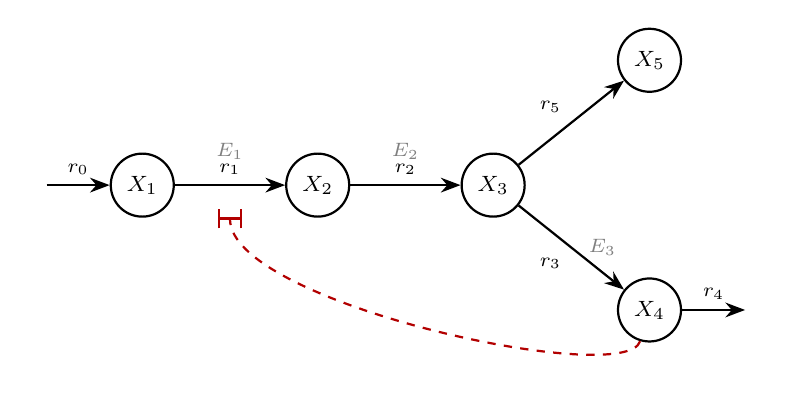
\begin{tikzpicture}[
        species/.style={circle, draw, thick, minimum size=8mm, font=\footnotesize},
        enzyme/.style={font=\scriptsize\itshape, text=gray},
        arr/.style={-{Stealth[length=2.5mm]}, thick},
        inh/.style={-{Tee Barb[length=2.5mm, width=3mm]}, thick, red!70!black, dashed},
        node distance=14mm
    ]
        \node[species] (X1) {$X_1$};
        \node[species, right=of X1] (X2) {$X_2$};
        \node[species, right=of X2] (X3) {$X_3$};
        \node[species, below right=10mm and 14mm of X3] (X4) {$X_4$};
        \node[species, above right=10mm and 14mm of X3] (X5) {$X_5$};

        \node[left=8mm of X1] (src) {};
        \node[right=8mm of X4] (sink) {};

        \draw[arr] (src) -- node[above, font=\scriptsize] {$r_0$} (X1);
        \draw[arr] (X1) -- node[above, font=\scriptsize] {$r_1$} (X2);
        \draw[arr] (X2) -- node[above, font=\scriptsize] {$r_2$} (X3);
        \draw[arr] (X3) -- node[below left, font=\scriptsize] {$r_3$} (X4);
        \draw[arr] (X3) -- node[above left, font=\scriptsize] {$r_5$} (X5);
        \draw[arr] (X4) -- node[above, font=\scriptsize] {$r_4$} (sink);

        \node[enzyme, above=2mm of {$(X1)!0.5!(X2)$}] {$E_1$};
        \node[enzyme, above=2mm of {$(X2)!0.5!(X3)$}] {$E_2$};
        \node[enzyme, right=1mm of {$(X3)!0.5!(X4)$}, font=\scriptsize\itshape, text=gray] {$E_3$};

        \draw[inh] (X4) .. controls +(-0.3,-1.0) and +(0,-1.2) .. ($(X1)!0.5!(X2)+(0,-0.3)$);
    \end{tikzpicture}

    \vspace{2mm}

    \includegraphics[width=0.85\textwidth]{figures/feedback_simulation.pdf}
    \caption{Dynamic simulation of a feedback-inhibited linear pathway. Top: reaction network where solid arrows denote mass flow and the dashed red line indicates feedback inhibition of $r_1$ by $X_4$. Bottom: concentration trajectories under a pulsed input $u_1(t)$; product $X_4$ exerts feedback inhibition on $r_1$, limiting upstream accumulation during both the high and medium pulses.}
    \label{fig:feedback}
\end{figure}

\subsection{Steady-state analysis of a branched pathway}\label{sec:ex-steadystate}
We next consider a branched pathway in which a source produces species $A$, which is converted to $B$, then to $C$, at which point the pathway branches: $C$ is converted to $D$ via reaction $r_3$ (catalyzed by enzyme $E_3$) or to $E$ via reaction $r_4$ (catalyzed by enzyme $E_4$). Both $D$ and $E$ are degraded by first-order reactions $r_5$ and $r_6$. Two feedback loops are present: $E$ inhibits $r_1$ ($g_{E,r_1} = -0.5$) and $D$ inhibits $r_2$ ($g_{D,r_2} = -0.5$). This network topology is common in amino acid and nucleotide biosynthesis, where branch point enzymes control the distribution of flux between competing product pathways.

To illustrate how enzyme levels at the branch point control metabolic flux distribution, we sweep the concentration of $E_3$ from 0.1 to 5.0 while holding $E_4 = 1.0$ fixed and compute the steady-state concentrations using the \texttt{steadystate} function. \Cref{fig:steadystate} shows the result. At low $E_3$, reaction $r_3$ is slow relative to $r_4$, so most flux is directed toward $E$; the steady-state concentration of $E$ exceeds 1.8 while $D$ is below 0.2. As $E_3$ increases, the flux redistributes: the $D$ and $E$ curves cross near $E_3 \approx 1$, and at high $E_3$ the situation reverses, with $D$ reaching approximately 1.7 and $E$ dropping below 0.4. The branch point metabolite $C$ decreases monotonically with increasing $E_3$, as it is consumed more rapidly. The upstream species $A$ and $B$ also adjust through the feedback loops, decreasing as the changing $D$ and $E$ levels modulate $r_1$ and $r_2$. This example demonstrates how \texttt{BSTModelKit.jl} can be used to explore the relationship between enzyme levels and steady-state flux distribution, a central concern in metabolic engineering.

\begin{figure}[ht]
    \centering
    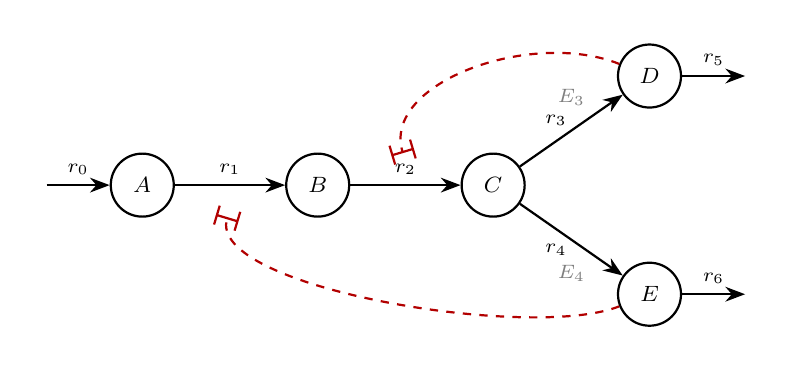
\begin{tikzpicture}[
        species/.style={circle, draw, thick, minimum size=8mm, font=\footnotesize},
        enzyme/.style={font=\scriptsize\itshape, text=gray},
        arr/.style={-{Stealth[length=2.5mm]}, thick},
        inh/.style={-{Tee Barb[length=2.5mm, width=3mm]}, thick, red!70!black, dashed},
        node distance=14mm
    ]
        \node[species] (A) {$A$};
        \node[species, right=of A] (B) {$B$};
        \node[species, right=of B] (C) {$C$};
        \node[species, above right=8mm and 14mm of C] (D) {$D$};
        \node[species, below right=8mm and 14mm of C] (E) {$E$};

        \node[left=8mm of A] (src) {};
        \node[right=8mm of D] (sinkD) {};
        \node[right=8mm of E] (sinkE) {};

        \draw[arr] (src) -- node[above, font=\scriptsize] {$r_0$} (A);
        \draw[arr] (A) -- node[above, font=\scriptsize] {$r_1$} (B);
        \draw[arr] (B) -- node[above, font=\scriptsize] {$r_2$} (C);
        \draw[arr] (C) -- node[above left=-1mm, font=\scriptsize] {$r_3$} (D);
        \draw[arr] (C) -- node[below left=-1mm, font=\scriptsize] {$r_4$} (E);
        \draw[arr] (D) -- node[above, font=\scriptsize] {$r_5$} (sinkD);
        \draw[arr] (E) -- node[above, font=\scriptsize] {$r_6$} (sinkE);

        \node[enzyme, above=2mm of {$(C)!0.5!(D)$}] {$E_3$};
        \node[enzyme, below=2mm of {$(C)!0.5!(E)$}] {$E_4$};

        \draw[inh] (E) .. controls +(-1.5,-0.6) and +(-0.3,-1.0) .. ($(A)!0.5!(B)+(0,-0.3)$);
        \draw[inh] (D) .. controls +(-1.5,0.6) and +(-0.3,1.0) .. ($(B)!0.5!(C)+(0,0.3)$);
    \end{tikzpicture}

    \vspace{2mm}

    \includegraphics[width=0.85\textwidth]{figures/steady_state_sweep.pdf}
    \caption{Steady-state analysis of a branched pathway with feedback inhibition. Top: reaction network where $C$ is converted to $D$ (via $r_3$, catalyzed by $E_3$) or $E$ (via $r_4$, catalyzed by $E_4$); dashed red lines indicate feedback inhibition of $r_1$ by $E$ and $r_2$ by $D$. Bottom: steady-state concentrations as a function of the enzyme level $E_3$. Increasing $E_3$ redirects flux from the $E$ branch to the $D$ branch; the two curves cross near $E_3 \approx 1$.}
    \label{fig:steadystate}
\end{figure}

\subsection{Global sensitivity analysis}\label{sec:ex-sensitivity}
Finally, we demonstrate the global sensitivity analysis capabilities of \texttt{BSTModelKit.jl} by identifying which parameters most influence the time-integrated concentration of $X_4$ in the feedback-inhibited pathway from \Cref{sec:ex-dynamic}. The seven parameters varied are the six rate constants $\alpha_{r_1}, \ldots, \alpha_{r_4}$ (with bounds at $\pm 50\%$ of their nominal values) and the feedback kinetic order $g_{X_4,r_1}$ (varied from $-2$ to $0$). The scalar performance metric is $J = \int_0^{20} X_4(t)\,dt$, representing the cumulative exposure to the product.

\Cref{fig:sensitivity} shows the results of both the Morris screening method (left panel, 500 trajectories) and the Sobol variance decomposition (right panel, 1000 quasi-random samples). The two methods yield consistent conclusions. The Morris elementary effects identify $\alpha_{r_0}$ (source rate) and $\alpha_{r_4}$ (product degradation rate) as the dominant parameters, with $\alpha_{r_5}$ (branch rate) a distant third; the upstream reaction rate constants and the feedback kinetic order have negligible influence. The Sobol analysis confirms this ranking: $\alpha_{r_4}$ has the largest first-order index ($S_1 \approx 0.54$) and total-order index ($S_T \approx 0.59$), followed by $\alpha_{r_0}$ ($S_1 \approx 0.38$, $S_T \approx 0.45$). The gap between $S_1$ and $S_T$ for both parameters indicates mild interactions, consistent with the multiplicative structure of the power-law kinetics. These results are intuitive: the integrated $X_4$ concentration is controlled primarily by how fast $X_4$ is produced (governed by the source feeding the pathway) and how fast it is removed (governed by $r_4$), while the intermediate conversion steps operate fast enough that their rate constants do not limit the overall accumulation.

\begin{figure}[ht]
    \centering
    \includegraphics[width=\textwidth]{figures/sensitivity_analysis.pdf}
    \caption{Global sensitivity analysis of the integrated $X_4$ concentration for the feedback-inhibited pathway shown in \Cref{fig:feedback}. Left: Morris screening identifies $\alpha_{r_0}$ and $\alpha_{r_4}$ as the most influential parameters based on mean absolute elementary effects. Right: Sobol variance decomposition confirms the ranking, with first-order indices ($S_1$) and total-order indices ($S_T$) shown for each parameter.}
    \label{fig:sensitivity}
\end{figure}

% ============================================================================ %
\section{Discussion}\label{sec:discussion}
We have presented \texttt{BSTModelKit.jl}, an open-source Julia package that provides a complete workflow for Biochemical Systems Theory modeling: declarative model specification in TOML or custom text formats, automated construction of the stoichiometric and kinetic order matrices, dynamic simulation via ODE integration, steady-state computation, and global sensitivity analysis using the Morris and Sobol methods. The package leverages the Julia scientific computing ecosystem---particularly \texttt{OrdinaryDiffEq.jl}, \texttt{SteadyStateDiffEq.jl} \citep{Rackauckas2017}, and \texttt{GlobalSensitivity.jl} \citep{Dixit2022}---to provide efficient and numerically robust solvers while maintaining a small, focused API. The three examples presented in \Cref{sec:examples} illustrate the range of analyses that can be performed: dynamic simulation of feedback-regulated pathways under time-varying inputs, systematic exploration of how enzyme levels at metabolic branch points control steady-state flux distribution, and identification of the most influential parameters through global sensitivity analysis.

Several limitations of the current implementation suggest directions for future development. First, \texttt{BSTModelKit.jl} currently supports only the S-system representation; extending the package to support the Generalized Mass Action (GMA) formalism would enable modeling of systems where aggregation of production and consumption terms into single power-law expressions is not appropriate, such as networks with multiple independent production pathways for a single species. Second, the package does not currently provide local sensitivity analysis; integration with Julia's automatic differentiation ecosystem (e.g., \texttt{ForwardDiff.jl}) would enable efficient computation of sensitivity coefficients and logarithmic gains, quantities that are central to the classical BST analysis framework \citep{Savageau1976,Voit2000}. Third, parameter estimation from experimental data is not yet supported; combining the power-law model structure with gradient-based optimization or Bayesian inference methods available in the Julia ecosystem would make it possible to calibrate BST models directly from time-series measurements. Finally, integration with \texttt{ModelingToolkit.jl} could enable symbolic simplification, automatic Jacobian generation, and compilation of optimized model code, further improving performance for large-scale systems. We anticipate that these extensions, together with the growing Julia ecosystem for scientific computing, will make \texttt{BSTModelKit.jl} a useful tool for researchers applying BST to problems in systems biology and metabolic engineering.

% ============================================================================ %
\section*{Acknowledgments}
This work was supported by NIH NHLBI R-33 HL 141787 and NIH NHLBI R01 HL 71944.

% ============================================================================ %
\section*{Data and Code Availability}
\texttt{BSTModelKit.jl} is freely available under the MIT license at \url{https://github.com/varnerlab/BSTModelKit.jl}. Documentation is available at \url{https://varnerlab.github.io/BSTModelKit.jl/dev/}.

% ============================================================================ %
\bibliographystyle{plainnat}
\bibliography{references}

\end{document}
